\chapter[Study III: Predictive Soundscape Modelling of the Lockdowns]{Investigating Urban Soundscapes of the COVID-19 Lockdown: A predictive soundscape modelling approach}

This paper is part of a special issue on COVID-19 Pandemic Acoustic Effects.

\section*{Abstract}
 The unprecedented lockdowns enforced around the world to fight COVID-19 in spring 2020 triggered changes in human activities in public spaces. A predictive modelling approach was developed to characterise the resulting change in the perception of the sound environment when people could not be surveyed. Building on a database of soundscape questionnaires ($N = 1,318$) and binaural recordings ($N = 693$) collected in 13 locations across London and Venice during 2019, new recordings ($N = 608$) were made in the same locations during the lockdowns in 2020. Using these 30-second-long recordings, linear multi-level models were developed to predict the pleasantness and eventfulness of the soundscapes during the lockdown and compare changes for each location. An online listening study also investigated the change in sound sources within the spaces. Results indicate:

 \begin{enumerate}
   \item human sounds were less dominant and natural sounds more dominant across all locations
   \item contextual information is important for predicting pleasantness but not for eventfulness
   \item in general, perception shifted towards less eventful soundscapes and to more pleasant soundscapes for traffic-dominated locations, but not for human- and natural-dominated locations.
 \end{enumerate}

 This study demonstrates the usefulness of predictive modelling and the importance of considering contextual information when discussing the impact of sound level reductions on the soundscape.

\section{Introduction}
 \label{sec:intro}
 The global emergency cause by the \gls{covid19} in early 2020 required national lockdown measures across the world, primarily targeting human activity. In the United Kingdom, construction and transport were allowed to continue, but a decrease in activity was observed \citep{Hadjidemetriou2020impact}. In other countries, such as Italy, the restrictions were more severe and even included limiting people's movement to a certain radius from their place of residence \citep{Ren2020Pandemic}. The explorations in environmental acoustics of lockdown conditions across the world have revealed various degrees of impact on the acoustic environment, both at a city-scale \citep{Asensio2020Changes,BonetSola2021Soundscape,Hornberg2021Impact,Munoz2020Lockdown,Rumpler2021Noise} and at a more local, public space-scale \citep{Aletta2020Assessing,AlsinaPages2021Changes,BonetSola2021Soundscape,VidaManzano2021sound}. In general, these studies have demonstrated a decrease in urban noise levels and indicated a difference in the amount of decrease depending on the type of space investigated (e.g. parks, urban squares, etc.) and the type of human activity characteristic for the space.

 Those studies were mostly focussed around the \gls{laeq}, as well as a standardization approach to reporting subsequent changes in soundscape proposed by \citet{Asensio2020Taxonomy}. They were not able to reveal the perceptual impact of such conditions in public spaces as well because of: 1) the lack of subjective data for the exact or comparable locations in previous years; and 2) the lack of participants present in public spaces during the lockdown, hence the ability to collect soundscape data in-situ. Attempts have been made to bridge this gap by using social networks to source subjective data, but this resulted in a focus on indoor conditions following the shift in the citizens' behaviour, i.e. spending more time indoors \citep{Bartalucci2021survey,Lee2021Attitudes}. \citet{GarridoCumbrera2021Perceptions} relied on an online survey deployed in England, Ireland, and Spain to explore the perceived change in natural environments in particular. They observed a consistent increase in the perceived presence of natural sounds across all major cities and rural areas respectively in these three countries. A very similar trend was observed in Argentina, also based on an online questionnaire without a listening task \citep{Maggi2021Perception}. By combining field recordings and focus groups, \citet{Sakagami2020How} and \citet{Lenzi2021Soundscape} observed changes in the sound source composition and the affective quality of soundscape in a residential area in Kobe, Japan and a public space in Getxa, Spain, respectively, during the different stages of the lockdown period. Following the easing of lockdown measures, a decrease in animal and traffic sounds was observed in Kobe, while an increase in eventfulness, loudness, and presence of human sound sources, followed by a decrease in pleasantness, was shown in Getxa.

 \citet{Aletta2020Assessing} explored the impacts of the \gls{covid19} lockdowns on the acoustic environment in London in particular, through many short-term (30s) binaural recordings. This study revealed that average reductions in the various locations considered ranged from 10.7 dB (\gls{laeq}) to 1.2 dB, with an overall average reduction of 5.4 dB. This metric-reporting focussed approach left the following research questions unanswered:
 \begin{enumerate}
   \item How would people have perceived these spaces as a result of this change in acoustic environment? (RQ1)
   \item Would these sound level reductions result in improvements to the soundscape of the spaces? (RQ2)
 \end{enumerate}

 The \nth{1} research question (RQ1), addressing the perceptual effect of the change in urban soundscape induced by the lockdowns, can be further broken down into the following questions:

 \begin{itemize}
   \item How was the sound source composition influenced by the change?
   \item How would the affective response to the acoustic environment in lockdowns change?
   \item Could this demonstrate the effect of human activities on the perception of an acoustic environment in general?
 \end{itemize}

 These questions arise out of the soundscape approach, which is characterised by prioritising the perceptual effect of an acoustic environment by taking into account the interaction of sound sources, context, and the person perceiving it \citep{ISO12913_1_2014IOS} \cit{truax1999}, bringing together objective and subjective factors. The soundscape approach to noise mitigation and management is being recognised as a response to arising environmental requirements on noise pollution and sustainability, such as the regulation of quiet areas in Europe \citep{EEA2020Environmental, Aletta2018Towards} \cit{Radicchi2021}. This has been further formalised in \citet{ISO12913_2_2018IOS} via the adoption of the circumplex model of soundscape \citep{Axelsson2010principal}, in which the perception of a soundscape can be described in terms of its pleasantness and eventfulness, as one of the standard methods of soundscape assessment.

 Soundscape research is therefore traditionally rooted in environmental acoustics and environmental psychology, typically dealing with outdoor spaces \citep{Torresin2020Indoor} and urban open spaces, where parks and squares are often used as case study sites \cit{Kang 2007}. A soundscape assessment typically requires people to be surveyed but the presence of people at a location influences assessment \citep{Aletta2018Towards} and 'quiet places' usually require low numbers of users to remain quiet, which limits the possibility of an assessment. Even in a crowded public space, soundscape surveys are demanding as they require significant resources to carry out at scale, limiting their widespread application \citep{Mitchell2020Soundscape}. Therefore, a need for a predictive model arises to overcome this limitation and improve the implementation of the soundscape approach into everyday planning and management practices.

 According to a recent review of predictive soundscape models from \citet{Lionello2020systematic}, the degree of employing auditory and non-auditory factors in soundscape prediction varies with some studies relying on contextual \citep{Kajihara2017Imaginary}, personal/demographic \citep{Erfanian2021Psychological} \cit{tarlao2021} or social media \citep{Aiello2016Chatty} data entirely to predict and generate soundscape features. Some methods also incorporate perceptually-derived features, such as subjective sound level and visual pleasantness as predictors \citep{Lionello2020systematic}, however this information must also be obtained from people via a survey and therefore are unsuitable for predictive modelling where surveys are not possible. This indicates the necessity for considering and accounting for the influence which contextual factors in a space have on the relationship between the sound environment itself and the listener's perception of it (i.e. the soundscape).

 Therefore, a third research question arises: what are the key features needed for a soundscape prediction model based on comprehensive acoustic on site measurements to be used for assessing locations with low social presence or in situations where conducting surveys is impractical (RQ3)?

\section{Materials and Methods}

 This study was conducted via initial onsite data collection campaigns in Central London and Venice in 2019 before the outbreak of \gls{covid19} as part of the \gls{ssid} project \citep{Mitchell2020Soundscape} and in 2020 during the strictest part of the lockdowns \citep{Aletta2020Assessing}, including objective acoustic data (2019 and 2020) and subjective responses (2019 only). Using both 2019 and 2020 binaural recordings, an online listening experiment was conducted to provide an understanding about the change in sound source composition. The 2019 onsite questionnaire data were used to define the dominant sound source at each location as a starting point for interpreting the soundscape change. A predictive model was developed to reveal the change in the perceived pleasantness and eventfulness using objective acoustic data and location to predict subjective responses. Although the initial (2019) dataset contains additional locations (specifically, in Spain, the Netherlands, and China), due to the nature of this study as a reaction to the strict movement and activity restrictions, the sites which could be included in the lockdown (2020) measurement campaigns were limited to locations where staff and equipment had access and where recordings could be undertaken during the spring of 2020.

 The sites were selected to provide a mixture of sizes and uses, varying in typology ranging from paved squares to small and large parks to waterside spaces across both cities. Throughout the text they are indexed via a LocationID based on the location's name (e.g. CamdenTown, SanMarco), while a more in-depth overview of each is given in supplementary files. %NOTE: Will need to adjust this within thesis.
 London is taken as an example of a large, typically noisy city while the Venice sample provides a unique look at spaces with typically very high human activity levels and no road traffic activity. In particular, the 2019 Venice surveys were taken to coincide with the yearly Carnevale festival in order to capture its distinct soundscape.

 The ISO/TS 12913 \citep{ISO12913_2_2018IOS} series were consulted for reporting on soundscape data. A detailed description of the 2019 survey campaigns in featured through the paper and in the supplementary files. This study was approved by departmental UCL IEDE Ethics Committee on \nth{17} July 2018 for onsite data collection and on the \nth{2} of June 2020 for the online listening experiment and is conducted in adherence to the ethical requirements of the Declaration of Helsinki \citep{WMA2013World}.

 \subsection{Onsite data: Questionnaires, binaural measurements, and recordings}
   %FIXME: Likely will not need this within thesis.
   The initial onsite data collection featured both questionnaire data collected from the general public and acoustic measurements, conducted across thirteen urban locations (in London $N=11$, in Venice $N=2$) between the \nth{28} of February and the \nth{21} of June 2019, with additional sessions in July and October 2019. A total of 1,318 questionnaire responses were collected from the general population across the measurement points during 1 -- 3 hour-long campaigns in both cities in 2019, accompanied by 693 approximately 30-second long 24-bit 44.1 kHz binaural recordings. Each of the 13 locations was characterised by between 14 to 80 recordings and between 32 to 155 questionnaire responses. Mean age of the participants was 33.9 (45\% male, 53.8\% female, 0.4\% non-conforming, 0.9\% prefer-not-to-say).

   The subsequent measurement campaign in 2020 mimicked the binaural recording strategy applied in the initial campaign and was performed between the \nth{6} and the \nth{25} of April 2020 in both cities, this time excluding the questionnaire. An additional 608 binaural recordings were collected on site in 2020.

   \subsubsection{Data collection}
   %FIXME: Probably don't need this section in thesis either.
   The 2019 data collection was performed across all the locations using the protocol based on the Method A of the ISO/TS 12913-2:2018 \citep{ISO12913_2_2018IOS}, as described in \citep{Aletta2020Assessing,Mitchell2020Soundscape}, collected either via handheld tablets or paper copies of the questionnaire. The full questionnaire and data collection procedure are given in \citet{Mitchell2020Soundscape}, however the key parts used for this study are those addressing sound source dominance and \gls{paq}.
   %NOTE: Skipping next section since it's detailed earlier in thesis.

   %NOTE: add a section to the methods about the projection. Heavy reference to / pulling from Lionello 2020 and JASA-EL paper.
   In order to simplify the results and allow for modelling the responses as continuous values, the 8 \gls{paq}s undergo a trigonometric projection to reduce them onto the two primary dimensions of pleasant and eventful, according to the procedure outlined in Part 3 of the ISO 12913 series \citep{ISO12913_3_2019IOS}. In order to distinguish the projected values from the Likert-scale \gls{paq} responses, the projected values will be referred to as \gls{isopl} and \gls{isoev} and can be considered to form an x-y coordinate point (x = \gls{isopl}, y = \gls{isoev}) as explained in detail in \citet{Lionello2021Introducing}.

   %NOTE: Skipping paragraph on binaural recording info

   \subsubsection{Data cleaning}
   %TODO: Move and expand this data cleaning section to the methods section
   The cleaning of the samples was conducted using the ArtemiS SUITE 11. The researcher discarded or cropped whole recordings, or its parts affected by wind gusts or containing noises and speech generated by the recording operator by accident or for the purpose of explaining the questionnaire to a participant. This resulted in 1,291 binaural recordings which were then processed further, as described in Section \ref{sec:analyses}. Psychoacoustic analyses are shown in supplementary files.

   In order to maintain data quality and exclude cases where respondents either clearly did not understand the \gls{paq} adjectives or intentionally misrepresented their answers, surveys for which the same response was given for every \gls{paq} (e.g. 'Strongly agree' to all 8 attributes) were excluded prior to calculating the ISO projected values. This is justified as no reasonable respondent who understood the questions would answer that they 'strongly agree' that a soundscape is pleasant and annoying, calm and chaotic, etc. Cases where respondents answered 'Neutral' to all \gls{paq}s are note excluded in this way, as a neutral response to all attributes is not necessarily contradictory. In addition, surveys were discarded as incomplete if more than 50\% of the \gls{paq} and sound source questions were not completed.
   %TODO: Update ISO citations to what we did in the ASA submission, that was better.
   The site characterisation per \citet{ISO12913_2_2018IOS} is available in the supplementary files, featuring the address, overall psychoacoustic characteristics of the location, typical use of each location, and pictures taken during the survey sessions.

   \subsubsection{Psychoacoustic analyses}
   \label{sec:analyses}
   %NOTE: May want to move this to methods as well.
   The binaural recordings were analysed in ArtemiS SUITE 11 to calculate the following suite of 11 acoustic and psychoacoustic features to be used as initial predictors:

   \begin{enumerate}
     \item Loudness (\gls{n5}, sones, per ISO 532-1:2017)
     \item Sharpness (\gls{s}, acum, per ISO 532-1:2017)
     \item Roughness (\gls{r}, asper)
     \item Impulsiveness (\gls{iu})
     \item Fluctuation Strength (\gls{fs}, vacil)
     \item Tonality (\gls{tu}, tuHMS)
     \item Zwicker Psychoacoustic Annoyance (\gls{pa}, per \citet{PsychoacousticsZwicker})
     \item \gls{laeq}, 30s (dB)
     \item \gls{la10la90} (dB)
     \item \gls{lcla} (dB)
     \item Relative Approach (\gls{ra}, per \citet{Genuit1996Objective})
   \end{enumerate}

   The (psycho)acoustic predictors investigated were selected in order to describe many aspects of the recorded sound -- in particular, the goal was to move beyond a focus on sound level, which currently dominates the existing literature on the acoustic effects of lockdowns noted in Section \ref{sec:intro}. In all, they are expected to reflect the sound level (\gls{laeq}), perceived sound level (\gls{n5}), spectral content (\gls{s}, \gls{lcla}, \gls{tu}), temporal character or predictability (\gls{iu}, \gls{fs}, \gls{ra}), and overall annoyance (\gls{pa}). These metrics have been proposed as indicators to predict perceptual constructs of the soundscape \citep{Aletta2017Dimensions, Aletta2016Soundscape} and have shown promise when combined together to form amore comprehensive model applied to real-world sounds \citep{Orga2021Multilevel}. The maximum value from the left and right channels of the binaural recording are used, as suggest in ISO/TS 12913-3:2019 \citep{ISO12913_3_2019IOS}.

   Table \ref{tab:corr} shows the Pearson correlation coefficient between each of the candidate acoustic features and the outcome pleasantness and eventfulness. For \gls{isopl} ($ISOPl$), we can perhaps see three tiers of correlations:

   \begin{enumerate}
     \item The more highly correlated tier ($|r| > 0.28$) consists of \gls{ra}, \gls{laeq}, \gls{r}, \gls{n5}, and \gls{pa}
     \item The low correlation tier consists of \gls{la10la90}, \gls{tu}, and \gls{iu}
     \item \gls{lcla}, \gls{iu}, and \gls{s} show no correlation
   \end{enumerate}

   For \gls{isoev} ($ISOEv$), these tiers are:
   \begin{enumerate}
     \item The more highly correlated tier ($|r| > 0.30$) consists of \gls{ra}, \gls{laeq}, \gls{tu}, \gls{r}, and \gls{n5}
     \item The low correlation tier consists of \gls{lcla}, \gls{la10la90}, \gls{fs}, and \gls{pa}
     \item \gls{iu} and \gls{s} show no correlation
   \end{enumerate}

   Among the correlations for the psychoacoustic metrics considered for inclusion as input features, we can see several highly inter-correlated features. As expected, \gls{pa}, \gls{laeq}, and \gls{n5} are highly correlated, meaning that careful consideration is paid to these features to ensure they do not contribute to multicollinearity in the final model.

 \subsection{Modelling}

   Two linear multi-level models (MLM) were computed to predict: 1) \gls{isopl}, and 2) \gls{isoev}. The inherent grouped structure of the \gls{ssid} database necessitates a modelling and analysis approach which considers the differing relationships between the objective acoustic features and the soundscape's perceived affective quality ratings across the various locations and contexts. The individual-level of the models is made up of the acoustic features calculated from the binaural recordings made during each respondent's survey period, while the group-level includes the categorical 'LocationID' variable indicating the location in which the survey was taken, acting as a non-auditory contextual factor.

   A separate backwards-step feature selection was performed for each of the outcome models in order to identify the minimal feature set to be used for predicting each outcome. In this feature selection process, an initial model containing all of the candidate features was fit. Each feature was then removed from the model one at a time, then the best-performing model is selected and the procedure continues step-wise until no improvement is seen by removing more features. This process is carried out first on the location-level features (including the potential to remove all features including LocationID, resulting in a 'flat' or standard multivariate linear regression model), then on the individual-level features. The performance criterion used for this process was the \gls{aic} \citep{Akaike1974New}. To check for multicollinearity among the selected features, the \gls{vif} was calculated and a threshold of $\gls{vif} < 5$ was set. Any features which remained after the backwards step-wise selection and which exceeded this threshold were investigated and removed if they were highly collinear with the other features.

   All of the input features are numeric values, in the units described above. Before conducting feature selection, the input features are z-scaled to enable proper comparison of their effect sizes. After the feature selection, the scaled coefficients are used in the text when reporting the final fitted models to facilitate discussion and comparison between the features. The unscaled model coefficients are reporting in \draft{Appendix B} to enable the models to be applied to new data. In order to properly assess the predictive performance of the model, an 80/20 train-test split with a balanced shuffle across LocationIDs was used. The z-scaling and feature selection were performed on the training set only, in order to prevent data leakage. To score the performance of the model on the training and testing sets, we use the \gls{mae}, which is in the scale of the response feature -- for \gls{isopl} and \gls{isoev} this means our response can range from $-1$ to $+1$. However, since the end-goal of the model is to predict the soundscape assessment of the location as a whole, rather than the individual responses, we also assess the performance of the model in predicting the average response in each location. To do this, the mean response value for each location is calculated, and the $R^2$ accuracy across LocationIDs is reported for both the training and testing sets.

   The model fitting and feature selection was performed using the `step` function from `lmerTest` (v3.1.3) \citep{Kuznetsova2017lmerTest} in R statistical software (v.4.0.3) \citep{RCT2021R}. The summaries and plots were created using the `sjPlot` package (v.2.8.6) \citep{Luedecke2021sjPlot} and `seaborn` (v.0.11.1) \citep{Waskom2021seaborn}.

 \subsection{Online Survey}

   A online listening test was conducted using the Gorilla Experiment Builder \href{www.275gorilla.sc}{} \citep{AnwylIrvine2020Gorilla}. The participants were exposed to a random selection of 78 binaural recordings (39 from 2019 and 39 from 2020, 6 recordings per location). Each participant had the option to evaluate either 1 or 2 sets of 6 recordings randomly assigned between 13 stimuli sets. Mp3 files, converted at 256 kBps were used due to the requirements of the Gorilla platform.

   No visual stimuli were used in the experiment. The experiment consisted of:

   \begin{enumerate}
     \item an initial exercise to enhance the chances of participants complying with the instructions and wearing headphones
     \item a training set using two randomly chosen binaural recordings (then not used in the main task) from the dataset
     \item a soundscape characterisation questionnaire starting with an open-ended question about perceived sound sources and featuring the same questions as the one used in-situ, looking into the perceived sound source dominance of the following four types: traffic noise, other noise, human sounds, and natural sounds
     \item a questionnaire on the basic demographic factors.
   \end{enumerate}

   The questionnaire used in Part 3 of the online experiment is report in \draft{Appendix A}.

   Having in mind the remote nature of the study and to ensure a minimum level of robustness for reliable sound source recognition, an initial exercise was performed consisting of a headphone screening test \citep{Woods2017Headphone} and a headphone reproduction level adjustment test \citep{Gontier2019Estimation}. The level adjustment was performed using an 11-second-long pink noise sample matched to the lowest and the highest \gls{la90} values from the experimental set. Participants were asked to adjust their listening level to clearly hear the quieter sample while keeping the level low enough, so they don't find the louder sample disturbing. The headphone screening test followed, featuring a stereo signal of 1-second-long 100 Hz sin tone, generated with Izotope RX6 application, played at a 3 dB difference where one of the equally loud pairs had its phase inverted. A 100 Hz sin was used because the pilot tests revealed that the 200 Hz sin tone proposed by \citet{Woods2017Headphone} created a higher uncertainty varying across different laptop models and would likely contribute to the chances of a participant fooling the test. It was expected that participants using speakers would not be able to either hear the sin wave or would be fooled by the inverted phase effect and therefore not able to pass the trials, unless they were indeed using headphones. The participant needed to recognise the quietest of the 3 samples in a trial of 6 attempts. Only participants correctly answering 5 or more out of 6 trials were allowed to proceed with the experiment. Participants were asked not to change their audio output settings during the rest of the experiment. This was introduced to ensure that a participant is using a headphone playback system which allows a listener to clearly recognise a 3 dB difference at 100 Hz as a proxy for sufficient audio quality playback.

   Online questionnaire data was collected between the \nth{9} of June and the \nth{9} of August 2020. Within the Gorilla Experiment Builder, a total of 250 attempts to complete the experiment were recorded, where 165 participants were excluded either on the basis of not passing the headphone screening ($N=79$) or for not completing the experiment, usually before engaging into the screening ($N=83$). Out of a total of 88 participants who completed the test, 2 participants were excluded as outliers as they provided uniform answers across all the questions and commented on not being able to properly hear the stimuli, despite their successful completion of the training tests. The participants of the online experiment were of mean age 32.42, 45.1\% male, 54.9\% female.

   Figure \ref{fig:lockdown-study-framework} illustrates and summarises the framework and sections described above.

   \begin{figure}
     \label{fig:lockdown-study-framework}
     \centering
     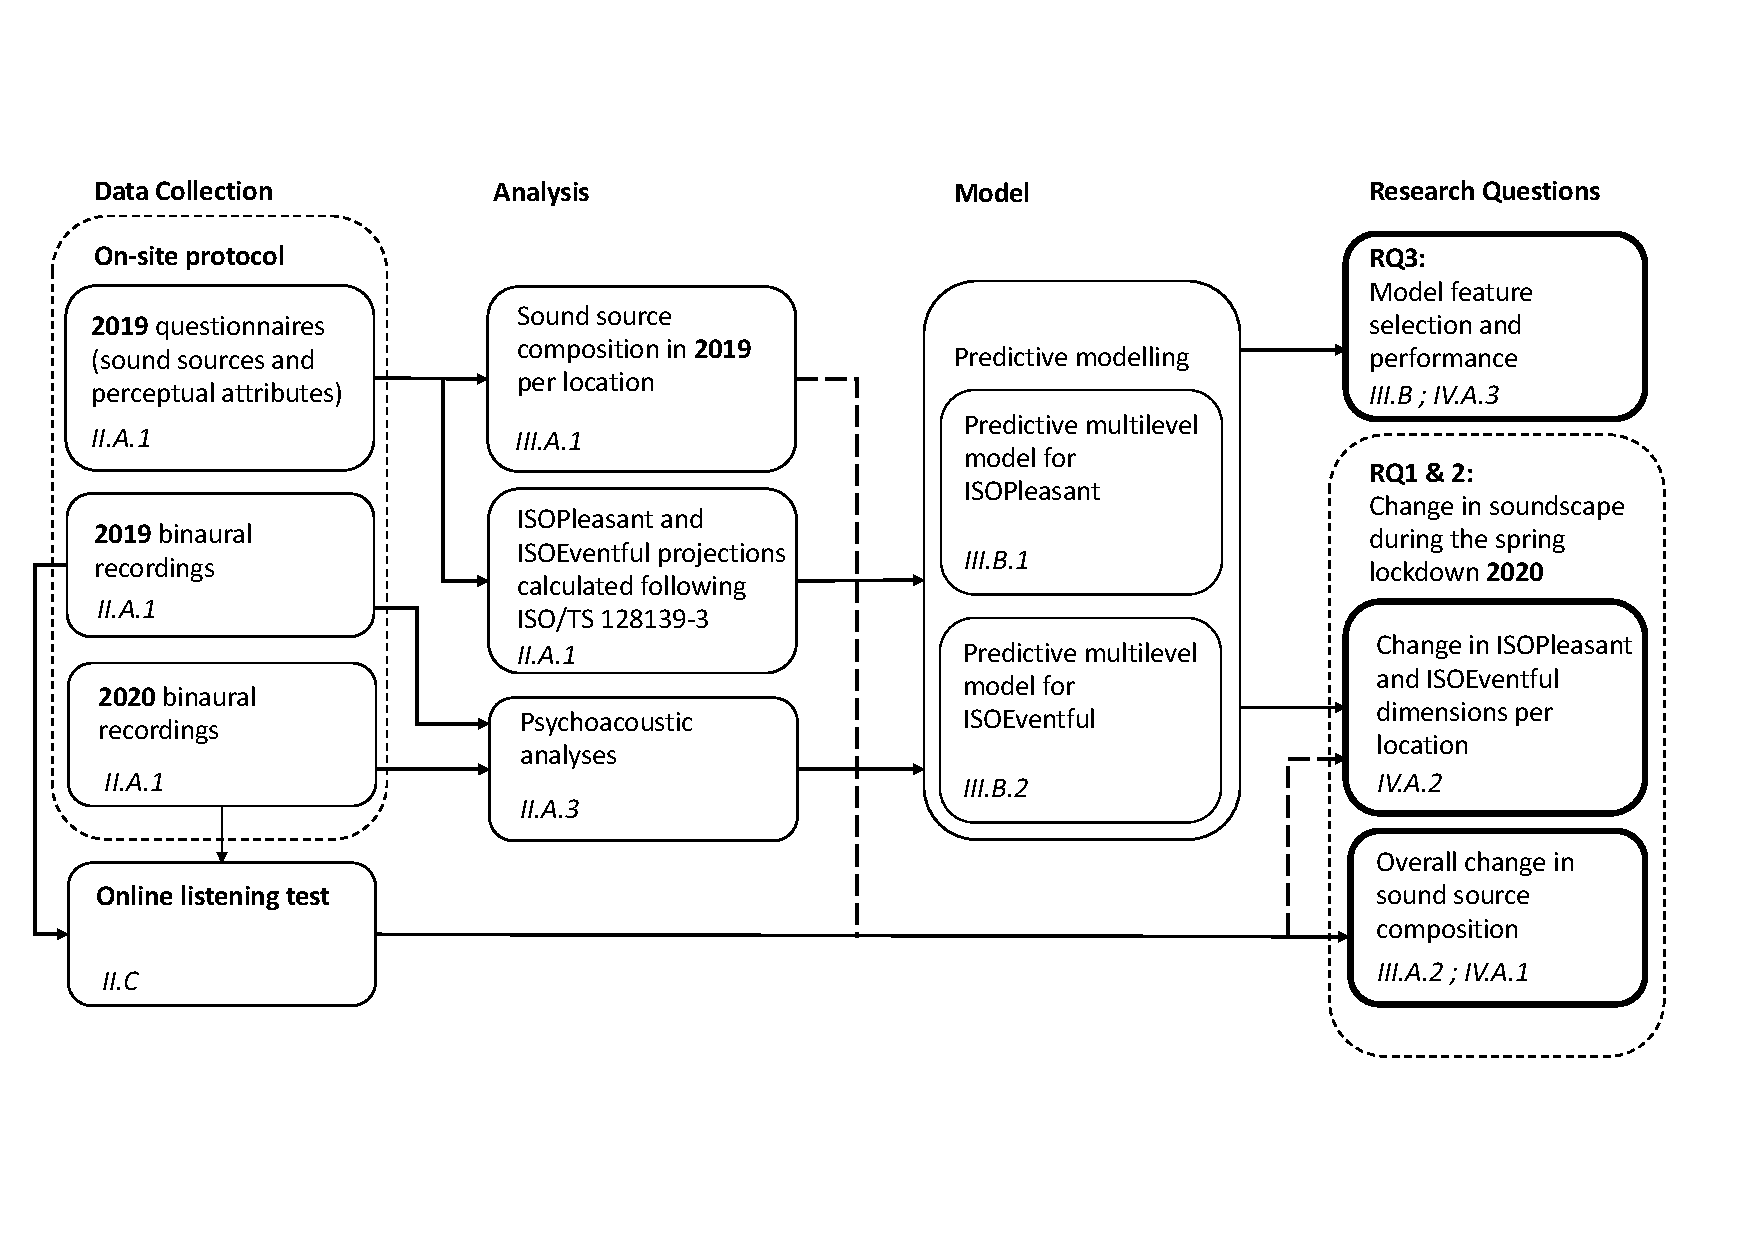
\includegraphics[width=\textwidth]{Figures/Lockdown-Fig1.pdf}
     \caption{The study flowchart indicating the data collection, analysis, modelling, and discussion throughout the study. The subsections in the text to which each box refers are indicated in italics.}
     %FIXME: Change the section references to match.
   \end{figure}

\section{Results}

 The results of the onsite surveys, online experiment, and the model development are reported here. They are reported following the structure of the ISO/TS 12913 series, revealing the perceived sound source dominance, key perceptual attributes (\gls{isopl} and \gls{isoev}) and the lockdown-related changes.

 \subsection{Perceived sound source dominance}

   \subsubsection{2019 sound source composition per location}

   Questionnaire data was collected English, Italian, and Spanish in both cities. The respective questionnaires can be found in the supplementary files and \citet{Mitchell2020Soundscape}. Data presented here was aggregated per LocationID.

   According to the highest scored mean value of the dominant sound source type, as show in Figure \ref{fig:sound-source-dom}, the locations can be grouped into: natural sounds dominated (RegentsParkJapan, RegentsParkFields, RussellSq), human sounds dominated (SanMarco, TateModern, StPaulsRow, StPaulsCross, MonumentoGaribaldi), noise (traffic and other noise) sounds dominated (CamdenTown, EustonTap, TorringtonSq, PancrasLock).

   \begin{figure}
     \label{fig:sound-source-dom}
     \centering
     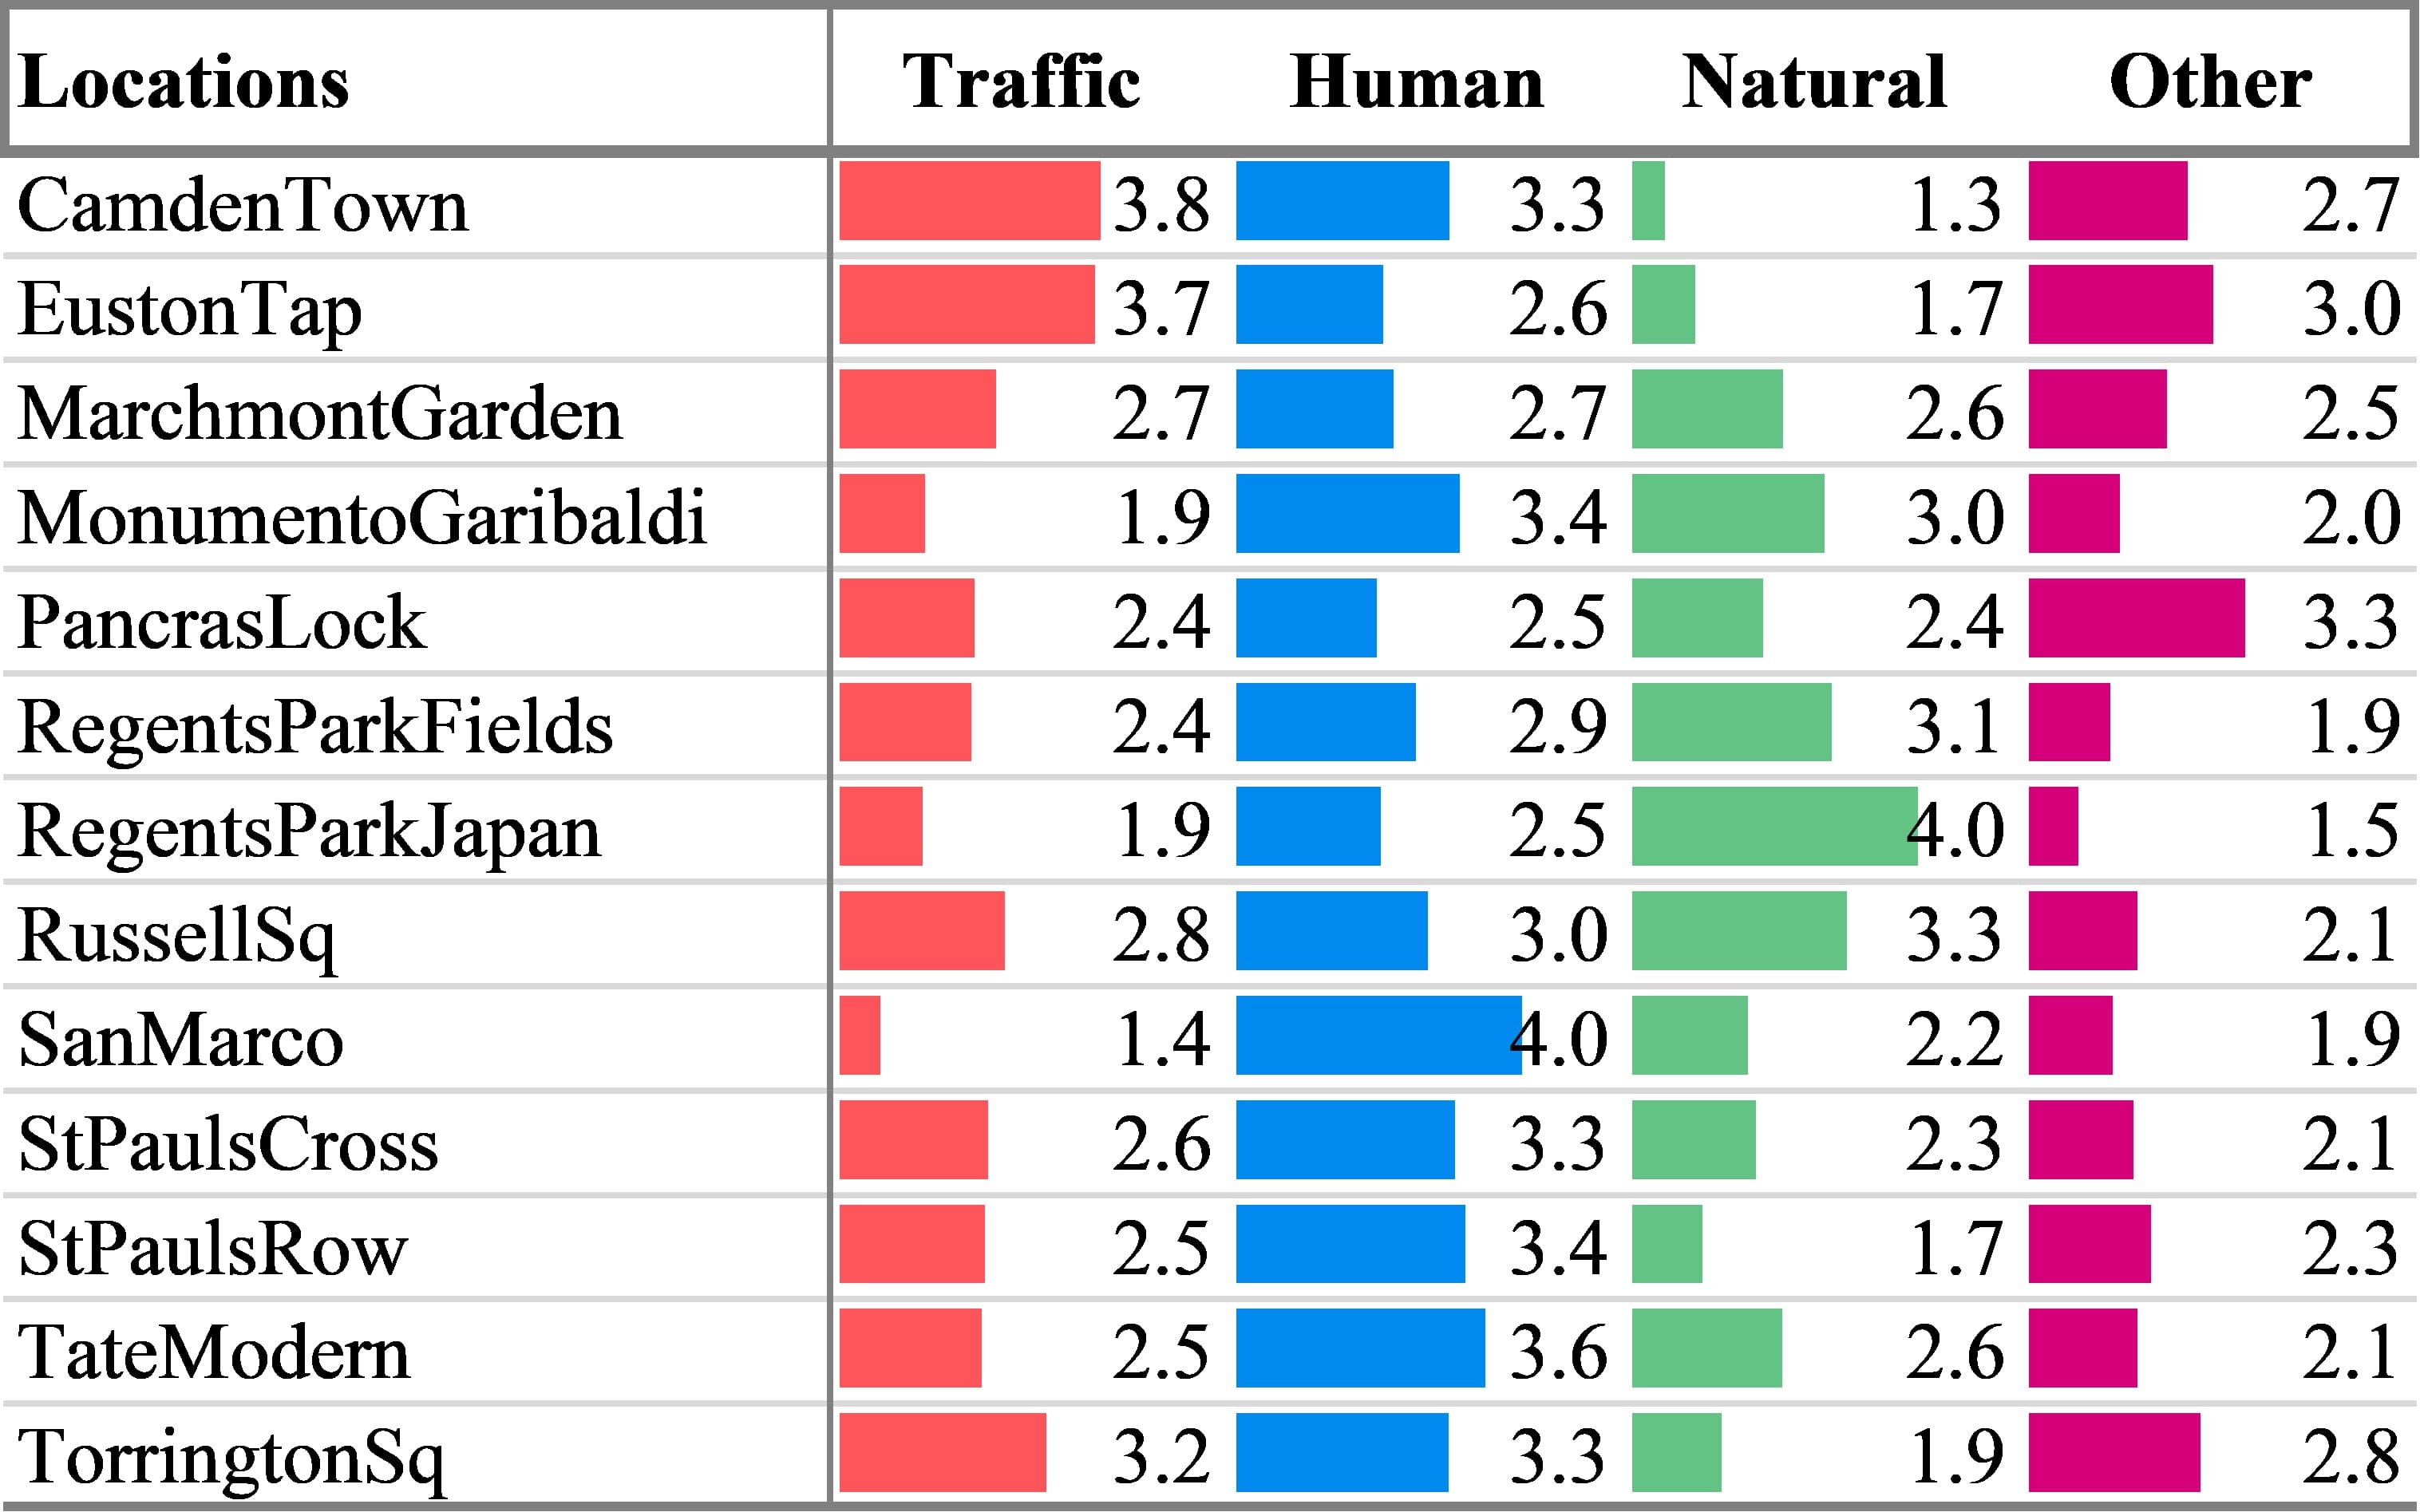
\includegraphics[width=.8\textwidth]{Figures/Lockdown-Fig2.jpg}
     \caption{Mean values per LocationID for the perceived dominance of the sound source types, for the 2019 on-site campaign.}
   \end{figure}

   \subsubsection{Overall change in the perceived sound source dominance during lockdown}

   1,803 words describing the sound sources present in the 2019 recordings and 1,395 words related to the 2020 recordings were input by participants in response to the open-ended question Q1 \draft{(see Appendix A)}. The frequency of occurrence, generated using the Word-Clouds web app, is shown in Figure \ref{fig:wordclouds}, for the 2019 and the 2020 sets respectively. The most frequency words from both 2019 and 2020 groups are: noise, car/traffic, bird/birds, talk/voice, and (foot)steps.

   \begin{figure}
     \label{fig:wordclouds}
     %TODO: add wordcloud figure
   \end{figure}

   The results from the listening tests deployed online were analysed using SPSS Statistics v. 25. Levene's test for equality of variances resulted in highly statistically significant values for all 4 sound sources investigated ($<0.001$). Therefore, a Mann-Whitney U-test was used as a non-parametric equivalent to the t-test to investigate the change in the perceived dominance of the four sound source types \citep{McKnight2010Mann}. The results for human sounds indicated that the perceived dominance was greater for the 2019 sample ($M=3.82$) than for the 2020 sample ($M=2.62, U=41,656, p<0.001$). The results for natural sounds indicated the perceived dominance increased from 2019 ($M=2.00$) to 2020 ($M=2.54, U=63,797, p<0.001$). However, the differences for the noise sources (traffic and other) were not statistically significant.

   \begin{figure}
     \label{tab:source-dominance-stats}
   \end{figure}

 \subsection{Model selection, performance, and application}

   \subsubsection{\gls{isopl} model selected}

   Following the feature selection, the \gls{isopl} model (given in Table \ref{tab:scaled-model}) has \gls{n5} as the fixed effect with a scaled coefficient of -0.06, and \gls{laeq}, \gls{la10la90}, and \gls{lcla} as coefficients which vary depending on the LocationID. The training and testing \gls{mae} are very similar, indicating that the model is neither over- nor under-fitting to the training data ($MAE_{train}=0.259, MAE_{test}=0.259$). The model performs very well at predicting the average soundscape assessment of the locations ($R^2_{train}=0.998, R^2_{test}=0.85$).

   \begin{table}
     \label{tab:scaled-model}
     \caption{Scaled linear regression models of \gls{isopl} and \gls{isoev} for 13 locations in London and Venice. The \gls{isopl} model is a multi-level regression model with one level for individual effects and a second level for LocationID effects, while the \gls{isoev} model is a 'flat' multi-variate linear regression with no location effects.}
   \end{table}

   The high intraclass correlation ($ICC=0.90$) demonstrates that the location-level effects are highly important in predicting the pleasantness dimension. Within this random-intercept random-slope model structure, these effects include both the specific context of the location (i.e. the LocationID factor), but also the \gls{laeq}, \gls{la10la90}, and \gls{lcla} features whose effects vary across locations. These slopes are given in Figure \ref{fig:pl-slopes}. This point highlights the need to consider how the context of a location will influence the relationship between the acoustic features and the perceived pleasantness.

   \begin{figure}
     \label{fig:pl-slopes}
     \caption{Location-level scaled coefficients for the \gls{isopl} model.}
   \end{figure}

   \subsubsection{\gls{isoev} model selected}

   Through the group-level feature selection, all of the group-level coefficients, including the LocationID factor itself. Therefore the final \gls{isoev} model is a 'flat' multi-variate linear regression model, rather than a multi-level model. The \gls{isoev} is a linear combination of \gls{s}, \gls{fs}, \gls{tu}, \gls{laeq}, and \gls{lcla}. The training and testing \gls{mae} are very similar, indicating that the model is not over-fit to the training data ($MAE_{train}=0.233; MAE_{test}=0.231$). The model performs slightly worse than the \gls{isopl} at predicting the mean location responses, but still performs well ($R^2_{train}=0.873; R^2_{test}=0.715$).

   \subsubsection{Application to lockdown data}
   %FIXME: Figure out how to do sub-figure referencing
   Once the two models were built and assessed, they were then applied to the lockdown recording data in order to predict the new soundscape ISO coordinates. Figure \ref{fig:circumplex-locations}(a) shows the pre-lockdown ISO coordinates for each location and Figure \ref{fig:circumplex-locations}(b) shows how the soundscapes are predicted to have been assessed during the lockdown period. As in the model assessment process, the predicted responses are calculated for each recording individually, then the mean for each location is calculated and plotted on the circumplex.

   In 2019 the majority of locations in the dataset fall within the 'vibrant' quadrant of the circumplex, particularly those which are primarily dominated by human activity (e.g. SanMarco, TateModern). CamdenTown and EustonTap, which are both in general visually and acoustically dominated by traffic, are the only two to be rated as 'chaotic', while no locations are overall considered to be 'monotonous'. During the 2020 lockdown, there is a general positive move along the 'pleasant' dimension and a general negative move along the 'eventful' dimension, but several patterns of movement can be noted. These are investigated further in the Discussion section below.

   \begin{figure}
     \label{fig:circumplex-locations}
     \caption{Soundscape circumplex coordinates for (a) the mean \gls{isopl} and \gls{isoev} responses for each location; and (b) the mean predicted responses based on recordings made during the lockdown and the location's movement in the circumplex.}
   \end{figure}

   %%%%%%%%%%%%%%%%%%%%%%%%%%%%%%%%%%%%%%%%%%%%%%%%%%%%%%%%%%%

\section{Discussion}

 \subsection{Interpretation of the results}

